\documentclass[10pt]{article}
\usepackage[margin=0.72in]{geometry}
\usepackage{amsmath,amssymb,amsthm,graphicx,microtype,caption}
\usepackage[colorlinks=true,linkcolor=black,urlcolor=blue!50!black]{hyperref}
\usepackage{titlesec}
\titleformat*{\subsection}{\normalsize\bfseries}
\titlespacing*{\subsection}{0pt}{6pt}{2pt}
\graphicspath{{../figures/}}
\captionsetup{font=small,labelfont=bf}
\pagestyle{empty}
\begin{document}
\begin{center}
{\Large\bfseries The Wrong Gradient: a two-page preview}\\[3pt]
Liam Kenji Bray \quad\textperiodcentered\quad full paper: \texttt{paper/main.pdf}
\end{center}

\subsection*{The setting}
Robots that each do what is best for themselves can make the group worse off. Four boats travel from a dock $S$ to an inspection area $T$; two canals (through junctions $A$ and $B$) take $2k$ minutes when $k$ boats use them, and two open legs take 10 minutes. Split two and two, the fleet spends 56 boat-minutes. Open a one-minute shortcut joining the canals and every boat, switching one at a time for its own benefit, ends on the zigzag route (canal, shortcut, canal) at 17 minutes each: the fleet spends 68 (Braess's paradox, price of anarchy $17/14$).

\subsection*{The central derivation}
With $n_e$ boats on edge $e$ and per-boat time $c_e(k)$, the fleet pays $C=\sum_e n_e\,c_e(n_e)$, while every selfish improvement (one boat switching routes to lower its own time) lowers Rosenthal's potential
\[
\Phi=\sum_e\sum_{k=1}^{n_e}c_e(k),\qquad\text{because a single boat's move changes }\Phi\text{ by exactly its own change in time.}
\]
Pictured on one edge, $\Phi$ is the \emph{area under a staircase} and $C$ is the \emph{rectangle} that encloses it: selfish boats minimize area while the fleet pays rectangles. The gap is the delay each newcomer imposes on the boats already there. Pricing that delay fixes it. Let $F_e(k)=k\,c_e(k)$ and charge each boat
\[
m_e(k)=F_e(k)-F_e(k-1)=c_e(k)+(k-1)\big[c_e(k)-c_e(k-1)\big].
\]
The potential $\Phi_m$ of the priced game, the analogue of $\Phi$ with $m_e$ in place of $c_e$, is then a telescoping sum, a discrete fundamental theorem of calculus:
\[
\Phi_m=\sum_e\sum_{k=1}^{n_e}\big[F_e(k)-F_e(k-1)\big]=\sum_e F_e(n_e)=C .
\]
In continuous form, $\tfrac{d}{dk}[k\,c(k)]=c(k)+k\,c'(k)$: my own delay plus what I add to each of the others.

\begin{figure}[h]
\centering
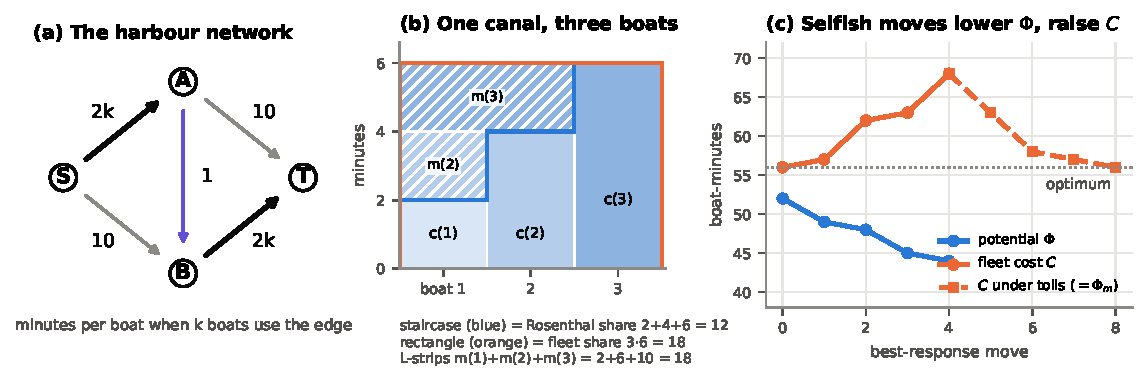
\includegraphics[width=0.86\linewidth]{fig1_braess.pdf}
\caption{(a) The harbour: dock $S$, inspection area $T$, junctions $A$ and $B$; violet is the shortcut. (b) One canal with three boats: staircase (Rosenthal's potential) inside the rectangle (fleet cost); the L-shaped strips are the marginal costs $m(k)$, and they telescope to the rectangle ($2+6+10=18$, against $2+4+6=12$ under the staircase). (c) Selfish moves lower $\Phi$ from 52 to 44 while $C$ rises from 56 to 68.}
\end{figure}

\subsection*{Potentials as conservative fields}
A game has an \emph{exact potential} if some function changes by exactly the mover's cost change whenever one player switches; a finite game has one if and only if, around every closed loop of four single-player moves ($i$ deviates, $j$ deviates, $i$ reverts, $j$ reverts), the movers' cost changes sum to zero (Monderer--Shapley). Writing $\Delta_i$ for the change when $i$ switches and $\Delta_j$ for the change when $j$ switches, that circulation equals $\Delta_i(\Delta_j c_j)-\Delta_j(\Delta_i c_i)$, a difference of mixed second differences, so the condition is a discrete version of $\partial F_x/\partial y=\partial F_y/\partial x$.

\subsection*{The boats are not a congestion game}
We built the harbour into a simulated robot-boat course with real dynamics (twin thrusters, drag, currents; RK4), calibrated $c_e(k)$ from the boats themselves, and solved the game exactly. The game predicted that opening the shortcut would cost the fleet 14\,s. The boats were \emph{6.7\,s faster} (100 paired random seeds, each fixing the currents, disturbances and start positions; 95\% confidence interval [5.6, 8.0]). The reason is that a single-file channel admits one boat every $h$ seconds, so boats leaving it reach the next channel already spaced out and barely queue. Delay depends on how traffic \emph{arrives}, not only on how much there is, which breaks the \emph{separable} form $c_e(n_e)$, in which each edge's cost depends only on its own load.

The four-cycle test makes this a theorem about the data. Using measured route costs in all 15 route profiles, the circulation around the 1{,}944 four-cycles is exactly zero for the calibrated game but reaches 21.7\,s for the measured one, six times the seed noise. Writing each boat's route as west (channel then open water), east (open water then channel) or shortcut, one loop of switches, (west, west, west, east) $\to$ boat 1 to east $\to$ boat 2 to shortcut $\to$ boat 1 back $\to$ boat 2 back, returns to its start with mover gains summing to $-21.7\pm0.7$\,s. The measured game even contains a strict improvement cycle, $(1,2,1)\to(2,1,1)\to(2,2,0)\to(1,2,1)$ in (west, east, shortcut) counts, every step gaining 3.6--10.8\,s. So the measured game has no ordinal potential (no function that even preserves the sign of every improvement) and no pure Nash equilibrium: selfish boats never settle. When congestion instead slows a group together (\emph{slow zones}, open water whose speed limit drops with the number of boats inside, rather than queues), coupling is weaker and the paradox appears: +63\,s measured against +43\,s predicted.

\begin{figure}[h]
\centering
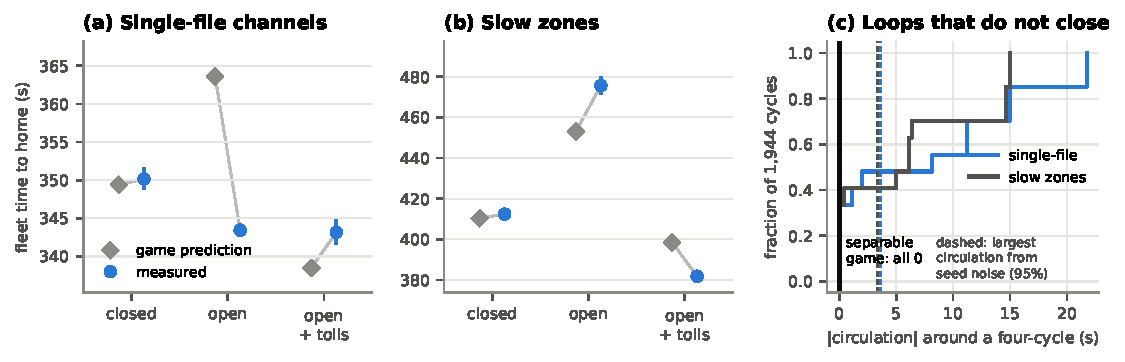
\includegraphics[width=0.8\linewidth]{fig_physical.pdf}
\caption{Prediction (grey diamonds) against measurement (blue dots, 95\% intervals) for single-file channels and slow zones; right, the distribution of circulation magnitudes of the measured games around all 1{,}944 four-cycles, with seed noise dashed; the calibrated congestion game is exactly zero on every one.}
\end{figure}

\subsection*{The research question}
\emph{When is a physical coordination problem well described by a potential game?} Here the separable model gets the sign of the paradox right only once the downstream bottleneck is about twice as slow as the upstream one, and the measured circulation gives a direct test. Three questions I would like to discuss:
\begin{enumerate}
\item Is there a natural congestion model with \emph{coupled} edges (queues in series) that still has a potential, perhaps over arrival schedules rather than routes?
\item Can a small measured circulation be turned into a bound, for instance that best responses still approximately descend some function with error proportional to the largest circulation? (Candogan et al.\ decompose games into potential and harmonic parts.)
\item The circulation is a mixed second difference; for players with continuous choices it becomes the antisymmetric part of a Jacobian. Does that view say anything about when gradient-like learning in robot teams converges?
\end{enumerate}
\end{document}
